\documentclass[a4 paper]{article}
% Set target color model to RGB
\usepackage[inner=2.0cm,outer=2.0cm,top=2.5cm,bottom=2.5cm]{geometry}
\usepackage{setspace}
\usepackage[rgb]{xcolor}
\usepackage{verbatim}
\usepackage{subcaption}
\usepackage{amsgen,amsmath,amstext,amsbsy,amsopn,tikz,amssymb}
\usepackage{fancyhdr}
\usepackage[colorlinks=true, urlcolor=blue,  linkcolor=blue, citecolor=blue]{hyperref}
\usepackage[colorinlistoftodos]{todonotes}
\usepackage{rotating}
\usepackage{tikz}
\usetikzlibrary{decorations.pathreplacing} 
\usepackage{float}
\usepackage{minted}


%\usetikzlibrary{through,backgrounds}
\hypersetup{%
pdfauthor={Ashudeep Singh},%
pdftitle={Homework},%
pdfkeywords={Tikz,latex,bootstrap,uncertaintes},%
pdfcreator={PDFLaTeX},%
pdfproducer={PDFLaTeX},%
}
%\usetikzlibrary{shadows}
% \usepackage[francais]{babel}
\usepackage{booktabs}
\newcommand{\ra}[1]{\renewcommand{\arraystretch}{#1}}

\newtheorem{thm}{Theorem}[section]
\newtheorem{prop}[thm]{Proposition}
\newtheorem{lem}[thm]{Lemma}
\newtheorem{cor}[thm]{Corollary}
\newtheorem{defn}[thm]{Definition}
\newtheorem{rem}[thm]{Remark}
\numberwithin{equation}{section}

\newcommand{\homework}[7]{
   \pagestyle{myheadings}
   \thispagestyle{plain}
   \newpage
   \setcounter{page}{1}
   \noindent
   \begin{center}
   \framebox{
      \vbox{\vspace{2mm}
    \hbox to 6.28in { {\bf 67800 - Probabilistic Methods in Artificial Intelligence \hfill {\small (#2)}} }
       \vspace{6mm}
       \hbox to 6.28in { {\Large \hfill #1  \hfill} }
       \vspace{6mm}
       \hbox to 6.28in { {\it Instructor: {\rm #3} \hfill TA: {\rm #5} \hfill Name: {\rm #6} {\rm #7}} }
       %\hbox to 6.28in { {\it TA: #4  \hfill #6}}
      \vspace{2mm}}
   }
   \end{center}
   \markboth{#6 -- #1}{#6 -- #1}
   \vspace*{4mm}
}

\newcommand{\problempoints}[2]{~\\\fbox{\textbf{Problem #1}}\hfill (#2 points)\newline\newline}
\newcommand{\subproblem}[1]{~\newline\textbf{(#1)}}
\newcommand{\D}{\mathcal{D}}
\newcommand{\Hy}{\mathcal{H}}
\newcommand{\VS}{\textrm{VS}}
\newcommand{\solution}{~\newline\textbf{\textit{(Solution)}} }

\newcommand{\important}[1]{\textcolor{blue}{\textit{\textbf{#1}}}} 

\newcommand{\problem}[1]{~\\\fbox{\textbf{Problem #1}} \newline\newline}


\newcommand{\bbF}{\mathbb{F}}
\newcommand{\bbX}{\mathbb{X}}
\newcommand{\bI}{\mathbf{I}}
\newcommand{\bX}{\mathbf{X}}
\newcommand{\bY}{\mathbf{Y}}
\newcommand{\bepsilon}{\boldsymbol{\epsilon}}
\newcommand{\balpha}{\boldsymbol{\alpha}}
\newcommand{\bbeta}{\boldsymbol{\beta}}
\newcommand{\0}{\mathbf{0}}

\setlength{\parindent}{0pt}


\begin{document}
\homework{Project 1 - Representation}{Due: 06/06/24}{Prof. Gal Elidan}{}{Hadar Tal}{}



\section{Warmup}


\section{Sampling}
\begin{enumerate}
    \item Use the sampling procedure described in the recitation to implement in the HMM class the method \texttt{sample}.
    \\ 
    \\
    \textcolor{blue}{
        Implemented the \texttt{sample} method in the \texttt{HMM} class.
    }

    \item Implement in the HMM class the method \texttt{log\_joint}, that calculates the joint probability for each sample \( p(X_{1:T}, O_{1:T}) \). 
    \\
    \\ \textcolor{blue}{
        Implemented the \texttt{log\_joint} method in the \texttt{HMM} class.
    }

    \item Sample \( N = 100 \) samples \( \xi^{[i]} = (X_{1:T}, O_{1:T}) \) from the HMM1 model with \( T = 1000 \). Calculate the joint probability of each sample \( p(\xi^{[i]}) \).
    \\
    \\ \textcolor{blue}{
        Loaded the HMM1 model and sampled \( N = 100 \) samples from the model with \( T = 1000 \).
    }
    \begin{minted}[fontsize=\footnotesize]{python}
        Load HMM1. CPDs:
        prior
        ['prior(0)=0.849' 'prior(1)=0.151']
        transition_mat
        [['tau(0->0)=0.750' 'tau(1->0)=0.250']
        ['tau(0->1)=0.250' 'tau(1->1)=0.750']]
        emission_mat
        [['e(0->0)=0.830' 'e(0->1)=0.170']
        ['e(1->0)=0.170' 'e(1->1)=0.830']]
    \end{minted}

    \textcolor{blue}{
        The log joint probabilities histogram is shown below.
    }    

    \item Plot the histogram of the log joint probabilities [*]. Why are the joint probabilities so small, even though the samples were sampled from the “correct” model?
    \\
    \begin{figure}[H]
        \centering
        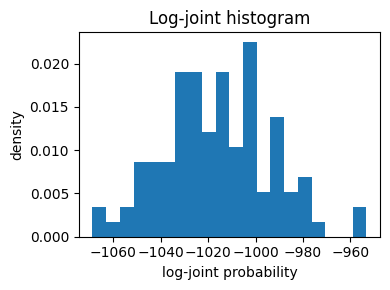
\includegraphics[width=0.45\textwidth]{../plots/Q2_hmm1_hist_log-joint.png}
    \end{figure}
    \textcolor{blue}{
        The joint probabilities are so small because they are the product of the prior, transition, and emission probabilities. 
        The transition matrix and the emission matrix are relatively far from the identity matrix. This implies that the randomness (or entropy) in the model is large, 
        meaning that the system transitions between states frequently and the observations can vary significantly. 
        As a result, each individual sequence of observations and hidden states becomes rare, leading to very small joint probabilities. 
        In essence, the higher the entropy, the more unique each sample is, which decreases the probability of any specific sample occurring.
    }

    
    \item Plot 3 examples of the sampled observations on top of the genome [*]. Plot a heatmap of all samples [*].
    \begin{figure}[H]
        \centering
        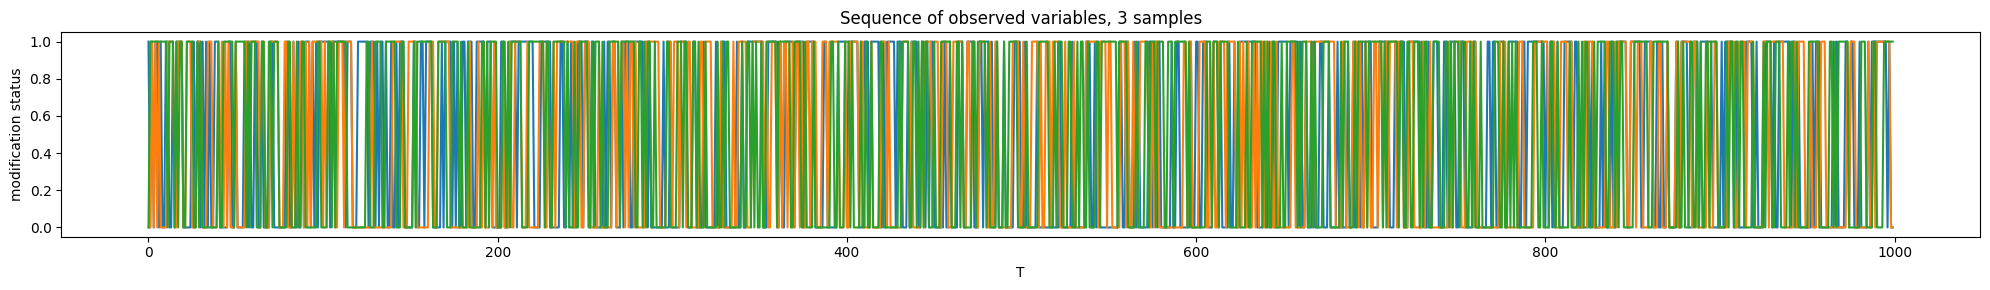
\includegraphics[width=\textwidth]{../plots/Q2_hmm1_sequence_observed.png}
    \end{figure}
    \begin{figure}[H]
        \centering
        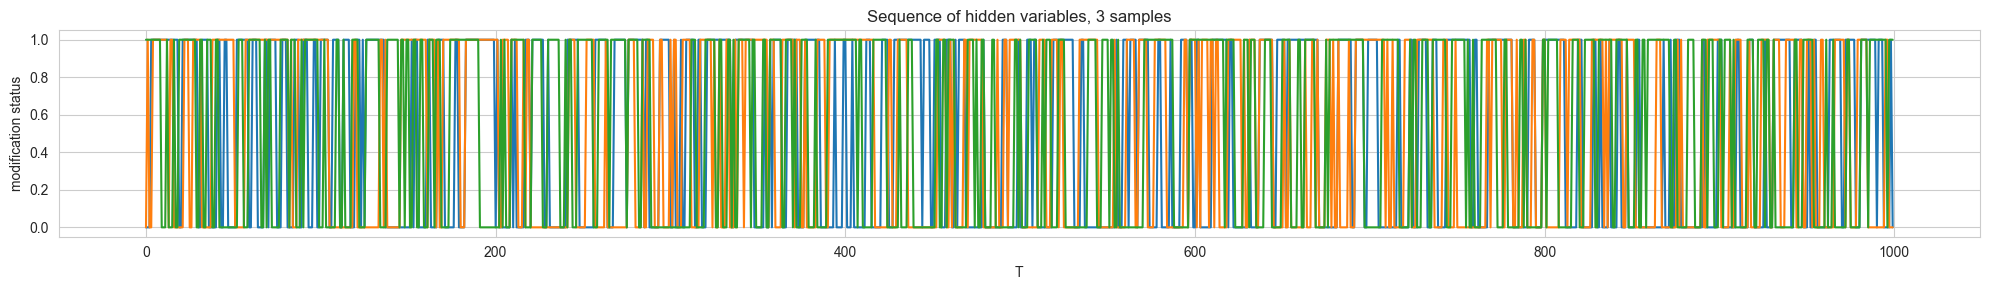
\includegraphics[width=\textwidth]{../plots/Q2_hmm1_sequence_hidden.png}
    \end{figure}    
    \begin{figure}[H]
        \centering
        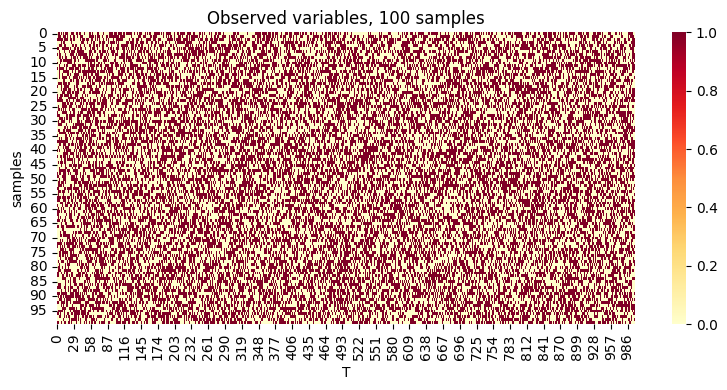
\includegraphics[width=0.55\textwidth]{../plots/Q2_hmm1_heatmap_observed.png}
    \end{figure}

    
    \item Do the same (3-5) for HMM2 with \( T = 1000 \). What are the differences? How can they be explained?
    \\
    \begin{minted}[fontsize=\footnotesize]{python}
        Load HMM2. CPDs:
        prior
        ['prior(0)=1.000' 'prior(1)=0.000']
        transition_mat
        [['tau(0->0)=0.999' 'tau(0->1)=0.001']
        ['tau(1->0)=0.005' 'tau(1->1)=0.995']]
        emission_mat
        [['e(0->0)=0.990' 'e(0->1)=0.010']
        ['e(1->0)=0.010' 'e(1->1)=0.990']]
    \end{minted}

    \begin{figure}[H]
        \centering
        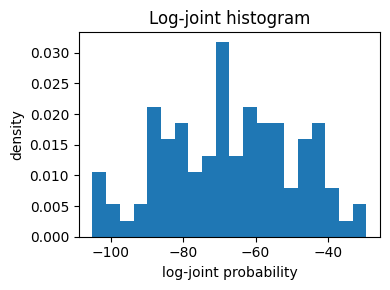
\includegraphics[width=0.45\textwidth]{../plots/Q2_hmm2_hist_log-joint.png}
    \end{figure}  
    \begin{figure}[H]
        \centering
        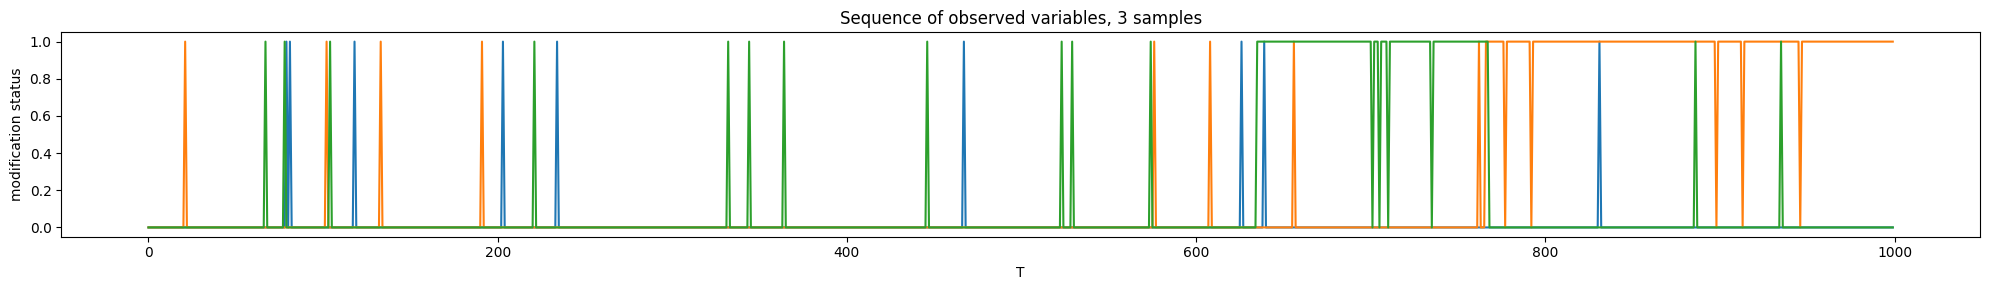
\includegraphics[width=\textwidth]{../plots/Q2_hmm2_sequence_observed.png}
    \end{figure}
    \begin{figure}[H]
        \centering
        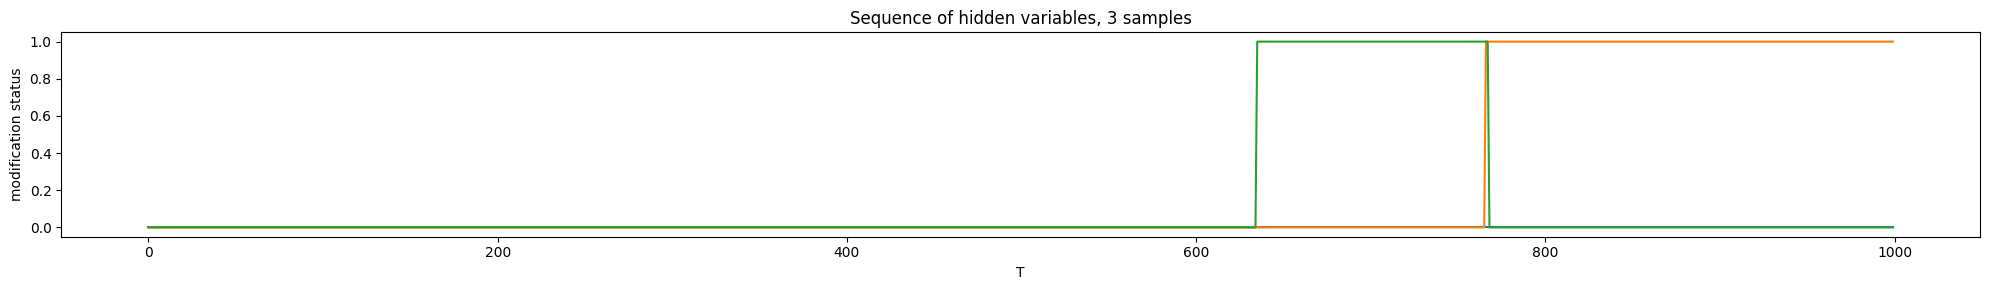
\includegraphics[width=\textwidth]{../plots/Q2_hmm2_sequence_hidden.png}
    \end{figure}    
    \begin{figure}[H]
        \centering
        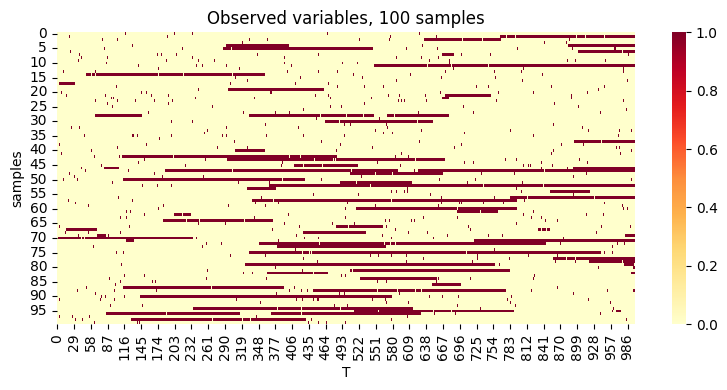
\includegraphics[width=0.55\textwidth]{../plots/Q2_hmm2_heatmap_observed.png}
    \end{figure}

    \textcolor{blue}{
        The differences between the results of HMM1 and HMM2 are evident in the log joint probabilities and the behavior of hidden and observed sequences: \\
        \begin{enumerate}
            \item \textbf{Log Joint Probabilities:}
            \begin{itemize}
                \item \textbf{HMM1:} Log joint probabilities are much smaller (more negative).
                \item \textbf{HMM2:} Log joint probabilities are higher (less negative).
            \end{itemize}
            \item \textbf{Hidden and Observed Sequences:}
            \begin{itemize}
                \item \textbf{HMM1:} Frequent transitions between states, indicating high randomness.
                \item \textbf{HMM2:} Fewer transitions, indicating more stability and persistence in states.
            \end{itemize}
        \end{enumerate}
        \textbf{Explanation}
        \begin{enumerate}
            \item \textbf{Transition and Emission Matrices:}
            \begin{itemize}
                \item \textbf{HMM1:} Matrices far from the identity matrix, implying high entropy (more randomness). This results in lower log joint probabilities due to the rarity of each sequence.
                \item \textbf{HMM2:} Matrices closer to the identity matrix, implying lower entropy (less randomness). This results in higher log joint probabilities because sequences are more predictable.
            \end{itemize}
            \item \textbf{Entropy and Probability Distribution:}
            \begin{itemize}
                \item \textbf{High Entropy (HMM1):} Greater randomness means lower probability for specific sequences, resulting in very negative log joint probabilities.
                \item \textbf{Low Entropy (HMM2):} Less randomness increases the probability for specific sequences, resulting in higher log joint probabilities.
            \end{itemize}
        \end{enumerate}
        In summary, HMM1’s higher entropy leads to more random and rare sequences with lower log joint probabilities, while HMM2’s lower entropy leads to 
        more stable and common sequences with higher log joint probabilities.
    }
    
    \item Load real observations from the \texttt{small\_binary\_data.csv} file [*]. Plot these observations same as the sampled data (3) [*]. 
    What is the pattern in the real data? Explain the differences. Does this data fit the HMM model assumptions?
    \begin{figure}[H]
        \centering
        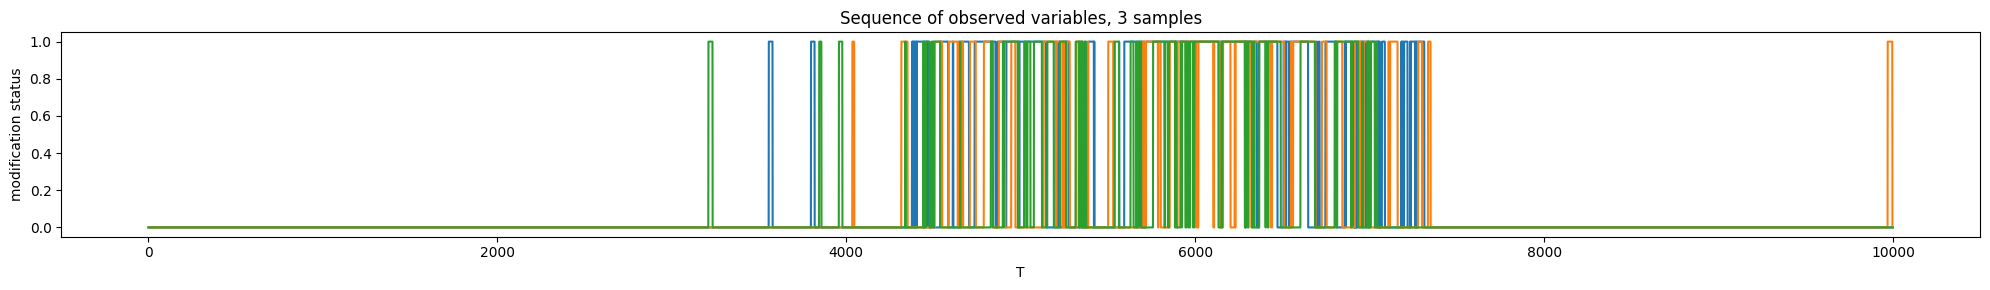
\includegraphics[width=\textwidth]{../plots/Q2_real_data_sequence_observed.png}
    \end{figure}
    \begin{figure}[H]
        \centering
        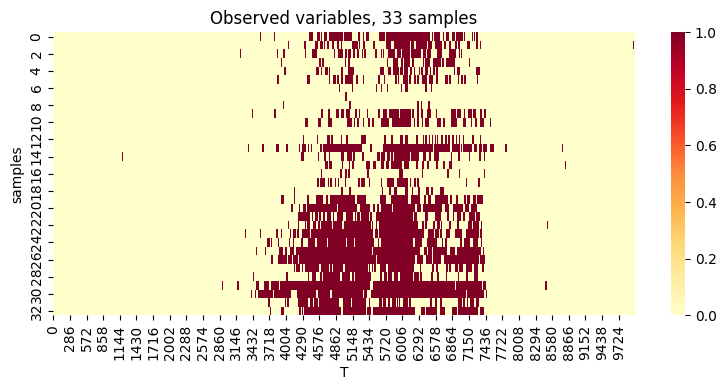
\includegraphics[width=0.45\textwidth]{../plots/Q2_real_data_heatmap_observed.png}
    \end{figure}  
    \textcolor{blue}{
        The real data from \texttt{small\_binary\_data.csv} shows a distinct pattern: many 1’s cluster in the middle of the sequence, while 0’s appear predominantly at the beginning and end. 
        This indicates the sequence does not follow the typical Markov properties assumed in HMMs. \\
        \textbf{Differences and Explanation}
        \begin{enumerate}
            \item \textbf{Pattern Differences:}
            \begin{itemize}
                \item \textbf{Real Data:} Clear structure with 1’s clustering in the middle and 0’s at the edges.
                \item \textbf{HMM Sampled Data:} More randomness and frequent state transitions, as expected from a Markov process.
            \end{itemize}
            \item \textbf{Explanation:}
            \begin{itemize}
                \item Real data exhibits non-Markovian behavior where state occurrences are not solely dependent on the previous state, indicating a structured or periodic phenomenon.
                \item This clustering pattern suggests that transitions between states are not memoryless, which is a fundamental assumption of HMMs.
            \end{itemize}
        \end{enumerate}
        The real data shows a clear deviation from HMM assumptions, evidenced by the structured clustering of states. 
        This suggests the real-world process generating this data has a different underlying mechanism than what an HMM can capture.
    }

\end{enumerate}

\section{Calculating Prior, Likelihood, and Posterior}
As we discussed above, calculating the priors, likelihoods, and posteriors is difficult. However, there are efficient ways to calculate these probabilities using Dynamic-Programming. These are examples of inference problems, which we’ll explore more in the next chapter of the course. For now, we’ll focus on calculating the prior \( p(X_t) \) for some \( t \):

\begin{enumerate}
    \item We define a subproblem for each \( t = 1, \ldots, T \) and \( k \in \text{Val}(X) \):
    \[
    P[t, k] = p(X_t = k)
    \]
    How can we calculate \( P[1, k] \) directly from the network CPDs?
    
    \item Using the multiplicative rule, we get a recursive formula for \( P \):
    \[
    P[t, k] = p(X_t = k) = \sum_{l \in \text{Val}(X)} p(X_t = k | X_{t-1} = l) \cdot p(X_{t-1} = l) = \sum_{l} p(X_t = k | X_{t-1} = l) \cdot P[t-1, l]
    \]
    Using this formula, we can iteratively fill a table \( P_{|\text{Val}(X)| \times T} \) by first filling the first column with the start conditions \( P[1, k] \), and continuing by columns: At each stage \( t \), we use the \( t \)-th column to compute the \( (t+1) \)-th. Implement in the HMM class the method \texttt{log\_p\_Xt}, that calculates the table \( \log P[t, k] = \log p(X_t = k) \).
    
    \item Implement in the HMM class the method \texttt{log\_p\_Xt\_given\_Ot}, that calculates \( \log p(X_t | o_t) \). Hint: How can you use \( \log p(X_t = k) \) to calculate the point-wise log posterior \( \log p(X_t | o_t) \)?
    
    \item Next, we supply you with a function \texttt{\_log\_forward} that calculates the log of the table \( \log F[t, k] = \log p(X_t = k, o_{1:t}) \) in a similar way to the log prior (we’ll talk about this algorithm later in the course) [*]. Implement in the HMM class a method \texttt{log\_likelihood}, that calculates the log-likelihood of the observations \( \log p(o_{1:m}) \).
\end{enumerate}

\section{Identifying Corrupt Data}
You are given a validation and a test dataset, each including a set of observations. The validation dataset was sampled directly from the HMM2 model. In the test dataset, the data is noisy, and some modification statuses were flipped (corrupted). We want to differentiate between samples with noisy observations and the rest. Intuitively, our trained Bayesian network should assign lower probability to corrupted observations and higher probability to the real ones. We can use this intuition to filter out corrupted data:

\begin{enumerate}
    \item Calculate the log-likelihood of each observation in the validation dataset (which includes only real observations) under the HMM2 model:
    \[
    \log p(o_{1:m})
    \]
    
    \item Compute the average \( \mu \) and the standard deviation \( \sigma \) of the log-likelihood on the validation dataset (average and std of \( \log p(o_{1:m}) \) over the validation set samples).
    
    \item Define a prediction rule: A sample with observations that have log-likelihood \( \log p(o_{1:m}) \) below three standard deviations of the average marginal log-likelihood, are classified as corrupted. That is,
    \[
    \text{if } \log p(o_{1:m}) < \mu - 3 \cdot \sigma \Rightarrow o_{1:m} \text{ is corrupted}
    \]
    This rule states that if a sample’s observations are very unlikely to originate from the same distribution as the validation data, then it is corrupted. In our case, “very unlikely” is translated to 3 standard deviations away from the mean. This practice follows a rule called The Empirical Rule.
    
    \item For each sample in the test dataset, calculate its log-likelihood and classify it as corrupted or real using the prediction rule.
    
    \item Plot the histogram of the log likelihood \( \log p(o_{1:m}) \) for the validation data [*]. On top of this histogram, plot two more histograms: One of the marginal log probability for the observations classified as “real”, and another for the observations classified as “corrupted” [*]. Explain the results.
\end{enumerate}

\section{Predict Active Promoters}
Say we want to predict the most likely segmentation to active promoters given a sequence of modifications. We’ll try to use the following rule:
\[
\forall t, \hat{X}_t = \arg \max_x p(X_t | O_t)
\]


% \begin{enumerate}
%     \item Implement this rule in the \texttt{naive_predict} method of the HMM class (use the point-wise posterior from Section 3).
%     \item Sample  N = 100  samples  \{\xi^{[i]}\}{i=1}^N  from HMM3 and predict their active promoter sequence  \{\hat{X}^{[i]}\}{i=1}^N .
%     \item Calculate the single-location accuracy of the prediction:

%     \text{single-location-accuracy} = \frac{1}{N \cdot T} \sum_{i=1}^N \sum_{t=1}^T \mathbf{1}\{ \xi^{[i]}_t = \hat{X}^{[i]}_t \}
%     What is the accuracy of the naive-predictor? Is this a good prediction rule? If not, suggest a better rule (no need to implement).
% \end{enumerate}




\end{document}